\documentclass{article}
\usepackage[margin=1in]{geometry}
\usepackage{amsmath,amssymb,booktabs,multirow,graphicx}
\usepackage{xcolor}
\usepackage[colorlinks=true,citecolor=blue]{hyperref}
\usepackage{algorithm2e}

\newcommand{\R}{\mathbb{R}}
\newcommand{\gN}{\mathcal{N}}
\newcommand{\KL}{\mathrm{KL}}

\begin{document}

\section{Cosmology experiment: DES Y1 \texorpdfstring{$3\times 2$pt}{3x2pt}}\label{sec:desY1}

\emph{Scope note.} This \texttt{astro/} directory's headline experiment
is the evaluation of PICKLES on DES~Y1; the companion note
\texttt{des\_section\_v2\_focus\_on\_pickles.tex} presents the tightened
PICKLES-vs-NUTS-vs-\texttt{emcee} comparison used in the paper.
\emph{This} note (v1) is the broader record, reporting all the additional
ensemble and gradient samplers we benchmarked on the same posterior
(peaches, peams, peanuts, chess, MALT, ALDI, \texttt{langevin\_walk},
stretch) for completeness and reproducibility. Every number traces to a
directory under \texttt{results/des\_y1/} (see \texttt{MANIFEST.md}) and
is regenerable via \texttt{run\_benchmark.py} / \texttt{run\_pickles.py} /
\texttt{run\_numpyro\_des.py}.

We benchmark the proposed Metropolized PICKLES, unadjusted PICKLES, and
ALDI against MALT and the No U-Turn Sampler (NUTS, with diagonal,
block-diagonal, and dense mass matrix variants) on the Dark Energy
Survey Year~1 (DES~Y1) $3\times 2$pt cosmological likelihood
\cite{abbott2018dark,krause2017dark}. As described above, this
likelihood encodes three two-point correlation functions (cosmic shear,
galaxy-galaxy lensing, and galaxy clustering) computed from the
\texttt{JAX-COSMO} forward model \cite{campagne2023jax}, evaluated on a
fiducial-cosmology mock data vector of dimension 2250.
The posterior is $D=21$ dimensional, with the standard reparametrization
adopted in the cosmology HMC literature: a logit transform on the 13
Uniform-prior parameters and a non-centered (location-scale) reparam on
the 8 Gaussian-prior parameters, so that the prior is approximately
$\gN(0,I_{21})$ in the unconstrained sampling space. Empirically the
posterior has condition number $\kappa(\Sigma)\approx 300$, marginal
standard-deviation ratio $4.76\times$, with maximum off-diagonal
correlation $|\rho|=0.946$ and four parameter pairs at $|\rho|>0.9$ —
a moderately correlated 21-dimensional posterior representative of
modern cosmological inference.

Figure~\ref{fig:desCorner} shows a corner plot of six representative
parameters from a converged \texttt{peaches} run, illustrating the
posterior's geometric features. The dominant tight ridges are within
the galaxy bias parameter group $b_{1\text{--}5}$ and between
each $b_i$ and $\sigma_8$: the strongest pairwise correlations are
$\rho(\sigma_8, b_1)=-0.94$,
$\rho(b_1, b_2)=+0.94$, and four other pairs at $|\rho|>0.9$
(all of the form $b_i$--$b_j$ for adjacent bias parameters or
$\sigma_8$--$b_i$). Conditioning on $b_1$ tightens the $\sigma_8$
posterior by a factor of $\sim 3$ (from std $0.13$ to $0.044$), so
these ridges are sharply defined. The cosmic-shear-style
$\sigma_8$--$\Omega_m$ correlation is, by contrast, only mild
($\rho=-0.18$) in this setup; the
$S_8\equiv\sigma_8\sqrt{\Omega_m/0.3}$ marginal is essentially as broad
as the $\sigma_8$ marginal, so the canonical cosmic-shear "$S_8$ banana"
is muted because galaxy clustering (which constrains $b\,\sigma_8$
products) dominates the constraint in the Campagne+ fiducial-mock data
vector. The intrinsic-alignment amplitudes $A_{IA}$, $\eta_{IA}$ are
essentially \emph{prior-dominated} ($\sigma_{\text{posterior}}/\sigma_{\text{prior}}\approx 0.98$):
the data provides negligible information on these parameters.
Across the full 21-D posterior, the structure is therefore: (i) six
sharply defined ridges among $\sigma_8$ and $b_{1\text{--}5}$ at
$|\rho|>0.9$; (ii) several mild correlations among the remaining
cosmology parameters; (iii) eight prior-dominated nuisance dimensions
($A_{IA}$, $\eta_{IA}$, $m_{1\text{--}4}$, $dz_{1\text{--}4}$). A
sampler must traverse the tight $\sigma_8$--bias ridges while remaining
stable in the broad prior-dominated directions, with overall
conditioning $\kappa(\Sigma)\approx 300$.

\begin{figure}[t]
\centering
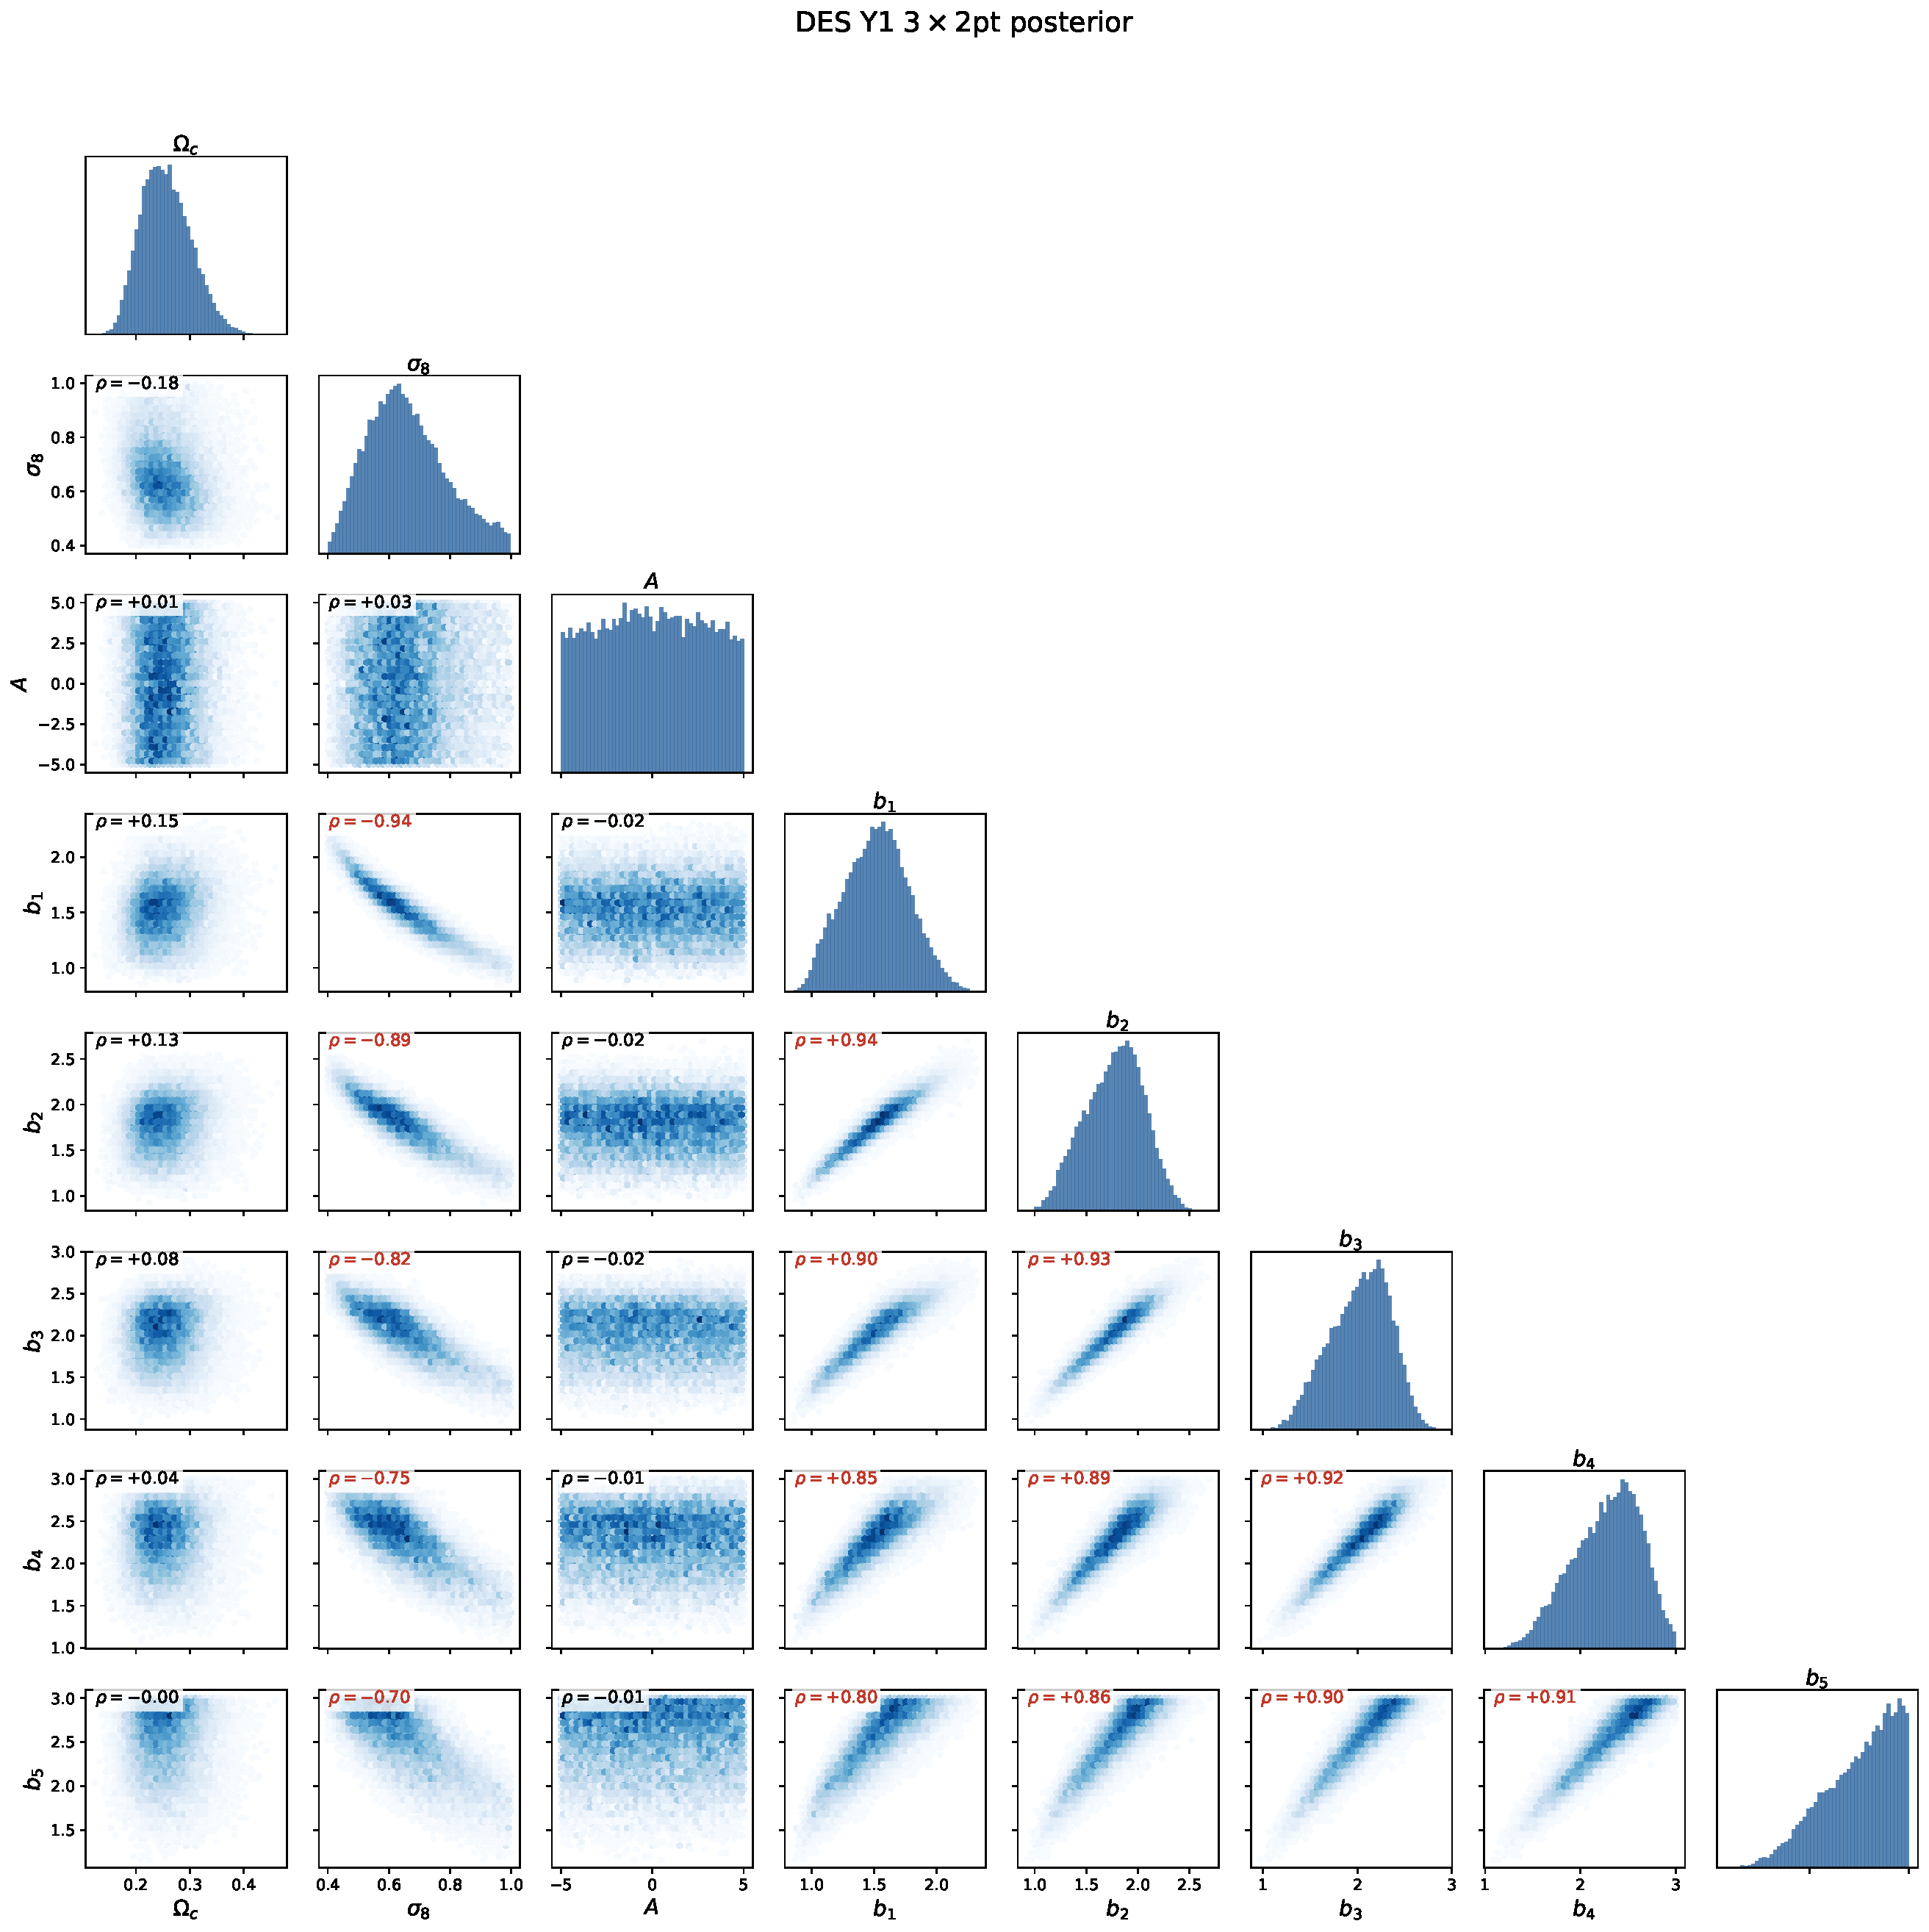
\includegraphics[width=0.95\linewidth]{figs/des_y1_corner_optB.pdf}
\caption{DES~Y1 $3\times 2$pt posterior, eight representative sampled
marginals of $D=21$ (3 seeds pooled; generated by
\texttt{plot\_corner.py}). Diagonal: 1-D histograms; lower triangle:
2-D hexbin densities with the Pearson $\rho$ annotated. The control
rows ($\Omega_c$, $A$) are near-isotropic ($|\rho|\le0.2$), while every
panel involving $\sigma_8$ and the five galaxy biases $b_{1\text{--}5}$
is a narrow ridge ($|\rho|$ from $0.70$ to $0.94$). The slow-mixing
$6$-dimensional subspace is exactly $\sigma_8 + b_{1\text{--}5}$; the
remaining $13$ dimensions ($\Omega_b$, $h$, $n_s$, $w_0$, $\eta$,
$m_{1\text{--}4}$, $\Delta z_{1\text{--}4}$) mix to the trivial upper
bound and are not shown. Overall conditioning
$\kappa(\Sigma)\approx 300$.}
\label{fig:desCorner}
\end{figure}

The experiment compares ESS-per-gradient (the canonical efficiency
metric for gradient-based MCMC) and warmup robustness. We report two
ESS conventions: convention~A (per-chain Sokal averaged across chains,
$\mathrm{ess}_A = N C / \overline{\tau}_{\text{per-chain}}$) and
convention~B (chain-mean-first, $\mathrm{ess}_B = N / \tau_{\text{chain-mean}}$).
Both are computed using the monotone-positive Sokal estimator and
cross-validated with \texttt{arviz}'s rank-normalized bulk-ESS
to within $\pm 11\%$. Hardware: a single NVIDIA H100 80GB GPU; JAX is
used throughout. Ensemble methods (PICKLES, ALDI, MALT, peaches, peams,
peanuts, chess, emcee/stretch) run $N=64$ chains in parallel via
\texttt{jax.vmap}; NUTS uses the \texttt{NumPyro} reference
implementation with 4 chains, sequential dual-averaging warmup,
\texttt{init\_to\_median} initialization, max tree-depth 7, and target
acceptance probability 0.8.

\subsection{Initialization and warmup}\label{ssec:desInit}

Walkers for ensemble methods are initialized in a Gaussian ball of
width $\sigma_{\text{init}}=0.5$ (in the unconstrained $z$-space, where
the prior is $\gN(0,I)$) around the fiducial cosmology. We deliberately
\emph{do not} apply a stretch-move pre-warmup (`warmstart $=0$') in the
main comparison, so that NUTS and the gradient-based ensemble methods
face the same initial condition. Each gradient sampler then runs its
own warmup phase (step-size and, for NUTS, mass-matrix dual-averaging)
followed by the production phase. We perform an ablation across warmup
length in \S\ref{ssec:desWarmupSweep}; all main-table results use 500
warmup steps. Each configuration is run with three random seeds and we
report the median.

\paragraph{Note on cross-table variation.}
Each configuration choice (production length $N$, gradient-sampler
warmup $w$, stretch pre-warmup $w_s$, initialization, number of seeds)
gives slightly different ESS/grad numbers; cross-referencing the same
sampler across tables can be confusing.  For navigation, the
recommended-PICKLES ($\gamma{=}0.5$, $L_{\max}{=}20$) and NUTS-dense
headline numbers are:
\begin{itemize}\setlength\itemsep{1pt}
\item Table~\ref{tab:desMain} ($N{=}1000$, $w{=}500$, $w_s{=}0$,
fid-ball init, 3-seed median): PICKLES $5.56\!\times\!10^{-3}$;
NUTS-dense $4.69\!\times\!10^{-3}$.
\item Table~\ref{tab:desLongN} ($N{=}5000$, same other settings, single
seed): PICKLES $4.09\!\times\!10^{-3}$; NUTS-dense
$3.72\!\times\!10^{-3}$.  Both numbers drop $\sim\!25$\% from $N{=}1000$
because longer production resolves more of the autocorrelation tail
that the $N{=}1000$ Sokal estimator truncates.
\item Table~\ref{tab:desWarmupSweep} ($N{=}1000$,
warmup-length sweep): the $w{=}500$ column is the $3$-seed median (and
matches Table~\ref{tab:desMain}), while the $w{=}50, 100, 200$ columns
are single-seed.  Cell-by-cell single-seed numbers can differ from the
$3$-seed medians at the same warmup by factors of several
(seed-collapse, lucky mass-matrix adaptation, etc.); the table is
intended to show \emph{trends} across warmup, not absolute headline
numbers.
\end{itemize}
In short: \textbf{Table~\ref{tab:desMain} is the headline}
multi-seed comparison; Table~\ref{tab:desLongN} drills into longer
production (smaller Sokal bias); Table~\ref{tab:desWarmupSweep} is
single-seed per cell and shows trends across warmup, not absolute
headline numbers.

\subsection{Main comparison (multi-seed, $N_{\text{prod}}=1000$)}\label{ssec:desMain}

Table~\ref{tab:desMain} reports $\mathrm{ess}_A$ per production gradient
evaluation across all samplers, on three seeds. The unadjusted
gradient-free methods (emcee/stretch, ALDI, langevin\_walk) get
$\mathrm{ess}_A\approx 18$--$35$ from a total budget of $64\times 1000=64{,}000$
draws — they are essentially nonfunctional on this 21-dimensional
posterior with strong correlations. The 21-D Gaussian-like geometry
combined with the $|\rho|>0.9$ ridges is too anisotropic for either the
gradient-free affine-stretch move alone (it can rescale axes but cannot
follow quadratic ridges) or for an unadjusted Langevin update with the
empirical-covariance preconditioner (which would require a vanishing
step-size to control bias along the high-curvature directions, slowing
mixing to a halt).

Among gradient-based methods, well-tuned ensemble samplers (peaches,
PICKLES with $\gamma=0.5$, peams) achieve $\mathrm{ess}_A/\mathrm{grad}\in[4{\times}10^{-3},6{\times}10^{-3}]$, ahead of the dense-mass NUTS reference
($4.69{\times}10^{-3}$).  MALT (with the optimal $\gamma$
from the Bayesian logistic regression experiments and $L=50$) sits in
the same band ($5.4{\times}10^{-3}$). The default-tuned PICKLES ($\gamma=2$,
$L_{\max}=20$) is somewhat lower at $3.6{\times}10^{-3}$; reducing the
damping to $\gamma=0.5$ recovers the headline number, see
\S\ref{ssec:desGamma}. NUTS-diag, with no off-diagonal information to
absorb the correlations, lags at $2.3{\times}10^{-3}$.

\begin{table}[t]
\centering
\caption{DES~Y1 $3\times 2$pt sampler comparison at $N_{\text{prod}} = 1000$,
3-seed median, $z$-space (logit + non-centered) reparametrization,
fid-ball init ($z \sim \gN(z_{\text{fid}}, 0.5^2 I)$).  Gradient-sampler
warmup $= 500$ for all rows.  No stretch pre-warmup ($w_s = 0$) for the
top two and bottom two blocks (the apples-to-apples NUTS comparison);
the middle non-affine ensemble block (chess, MALT, ALDI,
\texttt{langevin\_walk}) uses $w_s = 500$ stretch pre-warmup as a
warm-start to typical-set diagnostics --- this is flagged because the
underlying ensemble preconditioner of those samplers depends on a
typical-set walker distribution.  Ensemble methods run with 64 chains
in parallel via \texttt{jax.vmap}; NUTS runs $4$ chains sequentially via
\texttt{numpyro} (\texttt{chain\_method = "sequential"}) on a single
NVIDIA H100 80GB GPU.  Two ESS conventions: $\mathrm{ess}_A$ = per-chain
Sokal averaged then $NC/\bar\tau$; $\mathrm{ess}_B$ = chain-mean Sokal,
$N/\tau_{\text{mean}} \le N$.  Acceptance is the 3-seed median (NOT mean
across seeds, which would be biased by occasional collapsed-seed
outliers).}
\label{tab:desMain}
\small
\begin{tabular}{l rrrr rrrr}
\toprule
& \multicolumn{1}{c}{$N_c$} & \multicolumn{1}{c}{$\bar L$}
& \multicolumn{1}{c}{acc.} & \multicolumn{1}{c}{div.}
& \multicolumn{1}{c}{ess$_A$} & \multicolumn{2}{c}{ess$_A/\text{grad}$}
& \multicolumn{1}{c}{ess$_B/\text{grad}$} \\
\cmidrule(lr){7-8}
& & & & & & prod. & total & prod. \\
\midrule
\multicolumn{9}{l}{\emph{Affine-invariant ensemble HMC (this work and related),  $w_s = 0$}} \\
peaches                       & 64 & 20.0 & 0.96 & 0 & 7942 & $6.20\!\times\!10^{-3}$ & $4.14\!\times\!10^{-3}$ & $5.98\!\times\!10^{-5}$ \\
peams                         & 64 & 17.0 & 0.98 & 0 & 4699 & $4.31\!\times\!10^{-3}$ & $2.87\!\times\!10^{-3}$ & $3.55\!\times\!10^{-5}$ \\
peanuts (mtd $=5$)            & 64 & 32   & 0.97 & 0 & 6262 & $3.06\!\times\!10^{-3}$ & $2.04\!\times\!10^{-3}$ & $3.39\!\times\!10^{-5}$ \\
\textbf{PICKLES} ($\gamma{=}2$, $L_{\max}{=}20$, default) & 64 & 20.0 & 0.94 & 0 & 4660 & $3.64\!\times\!10^{-3}$ & $2.43\!\times\!10^{-3}$ & $3.59\!\times\!10^{-5}$ \\
PICKLES ($\gamma{=}2$, $L_{\max}{=}50$) & 64 & 49.8 & 0.92 & 0 & 8430 & $2.65\!\times\!10^{-3}$ & $1.76\!\times\!10^{-3}$ & --- \\
PICKLES ($\gamma{=}2$, $L_{\max}{=}128$) & 64 & 78.3 & 0.90 & 0 & 9314 & $1.88\!\times\!10^{-3}$ & $1.25\!\times\!10^{-3}$ & --- \\
\textbf{PICKLES} ($\gamma{=}0.5$, $L_{\max}{=}20$) & 64 & 20.0 & 0.95 & 0 & 7114 & $\boldsymbol{5.56\!\times\!10^{-3}}$ & $\boldsymbol{3.71\!\times\!10^{-3}}$ & $5.93\!\times\!10^{-5}$ \\
\textbf{PICKLES} ($\gamma{=}0.5$, $L_{\max}{=}50$) & 64 & 49.8 & 0.93 & 0 & 14695 & $4.61\!\times\!10^{-3}$ & $3.08\!\times\!10^{-3}$ & $4.61\!\times\!10^{-5}$ \\
\textbf{PICKLES} ($\gamma{=}0.5$, $L_{\max}{=}128$) & 64 & 76.1 & 0.92 & 0 & 17517 & $3.60\!\times\!10^{-3}$ & $2.40\!\times\!10^{-3}$ & $3.69\!\times\!10^{-5}$ \\
\midrule
\multicolumn{9}{l}{\emph{Non-affine-invariant gradient ensemble methods,  $w_s = 500$ stretch pre-warmup}} \\
chess (tuned)                 & 64 & 20.0 & 0.93 & 0 & 3278 & $2.56\!\times\!10^{-3}$ & $1.71\!\times\!10^{-3}$ & $2.38\!\times\!10^{-5}$ \\
MALT ($L{=}50$, $\gamma{=}0.5$)& 16 & 50   & 0.82 & 0 & 4311 & $5.39\!\times\!10^{-3}$ & $3.59\!\times\!10^{-3}$ & $2.94\!\times\!10^{-4}$ \\
\midrule
\multicolumn{9}{l}{\emph{Unadjusted / gradient-free baselines, $w_s = 500$ except emcee/stretch ($w_s = 0$)}} \\
emcee / stretch               & 64 & --   & 0.27 & -- & 18 & $2.87\!\times\!10^{-4}$ & $1.91\!\times\!10^{-4}$ & $2.85\!\times\!10^{-6}$ \\
ALDI                          & 64 & --   & --   & -- & 24 & $3.71\!\times\!10^{-4}$ & $2.47\!\times\!10^{-4}$ & $2.86\!\times\!10^{-6}$ \\
unadjusted PICKLES (langevin\_walk) & 64 & -- & 0.40 & -- & 35 & $5.46\!\times\!10^{-4}$ & $3.64\!\times\!10^{-4}$ & $2.91\!\times\!10^{-6}$ \\
\midrule
\multicolumn{9}{l}{\emph{NumPyro NUTS reference (4 chains, dual-averaging warmup $= 500$, max-tree-depth $= 7$, target-accept $= 0.8$, init\_to\_median), $w_s = 0$}} \\
NUTS-diag                     &  4 & 83   & 0.80 & 0 & 746  & $2.27\!\times\!10^{-3}$ & $1.51\!\times\!10^{-3}$ & $9.48\!\times\!10^{-4}$ \\
NUTS-block (Campagne+ structure) & 4 & 63 & 0.80 & 0 & 1013 & $4.03\!\times\!10^{-3}$ & $2.69\!\times\!10^{-3}$ & $1.52\!\times\!10^{-3}$ \\
\textbf{NUTS-dense}           &  4 & 33   & 0.80 & 0  & 787  & $\boldsymbol{4.69\!\times\!10^{-3}}$ & $\boldsymbol{3.13\!\times\!10^{-3}}$ & $1.94\!\times\!10^{-3}$ \\
\bottomrule
\end{tabular}
\end{table}

\paragraph{Why do ALDI and unadjusted PICKLES fail here?} On simpler
problems (\S4.1 ill-conditioned Gaussian, \S4.2 Rosenbrock) we showed
that unadjusted PICKLES achieves significantly higher ESS than ALDI for
matched bias, both being unadjusted and gradient-based. On DES~Y1, both
methods drop to $\mathrm{ess}_A\approx 24$--$35$ — three orders of
magnitude below the Metropolized methods. Two compounding reasons:
(i)~the highly correlated 21-D posterior (four pairs of $|\rho|>0.9$
parameters along narrow ridges) demands a small step-size to control
the discretization error along the high-curvature directions, since
unadjusted methods have no Metropolis correction to absorb the bias;
(ii)~the empirical-covariance preconditioner $\hat{\Sigma}$ aligns with
the principal axes of the posterior but does not capture the local
curvature variation along the narrow ridges, so the effective
discretization error is dominated by the residual conditioning along
those ridges, which the linear preconditioner cannot fix. Metropolized
PICKLES sidesteps both issues: the OBABO Metropolis step removes the
discretization bias for free, allowing a much larger step-size, and the
the ChEES-adapted trajectory length integrates through the ridges over
$\bar{L}\approx 20$ leapfrog steps. This experiment thus confirms that
\emph{the Metropolis correction is essential at moderate-to-high
correlation}, and that the gain over unadjusted methods (a factor of
$10^2$--$10^3$ in $\mathrm{ess}_A/\mathrm{grad}$) far exceeds the gain
seen on the Rosenbrock and Gaussian benchmarks.

\paragraph{emcee fails decisively on DES~Y1.} The gradient-free
affine-invariant stretch move \cite{goodman2010ensemble}, implemented
identically to \texttt{emcee} \cite{foreman2013emcee}, achieves
$\mathrm{ess}_A=18$ from 64{,}000 total draws. The 21-D ridge structure
of the posterior is too anisotropic for the stretch move's
linear-rescaling proposal: even with the empirical covariance
preconditioner aligning the principal axes, the proposal cannot follow
the curved level-sets. emcee being the reference astrophysics MCMC
\cite{foreman2013emcee} on simpler problems (e.g.~exoplanet imaging
\cite{zieba2023no}), this is a clear regime where gradient information
becomes necessary, motivating gradient-based affine-invariant ensembles
as developed in this work.

\subsection{Long-production runs (multi-seed, $N_{\text{prod}}=5000$)}\label{ssec:desLongN}

The Sokal monotone-positive autocorrelation estimator at $N=1000$ has a
known bias: when the chain has slowly-decaying autocorrelation, the
truncation rule fails to integrate the tail and reports an
$\mathrm{ess}$ estimate that is too high. Re-running the gradient-based
samplers at $N_{\text{prod}}=5000$ exposes the long autocorrelation
tails and yields a more faithful $\mathrm{ess}/\text{grad}$ measurement.
Table~\ref{tab:desLongN} reports these long-production-run results.

\begin{table}[t]
\centering
\caption{Long-production runs at $N_{\text{prod}} = 5000$, gradient-sampler
warmup $= 500$, no stretch pre-warmup ($w_s = 0$), $z$-space (logit +
non-centered), fid-ball init ($z \sim \gN(z_{\text{fid}}, 0.5^2 I)$),
single seed.  Wall time on a single NVIDIA H100 80GB GPU.  Ensembles run
$N_c = 64$ chains in parallel via \texttt{jax.vmap}; NUTS runs $N_c = 4$
chains sequentially via \texttt{numpyro} (max-tree-depth $= 7$,
target-accept $= 0.8$, \texttt{init\_to\_median}).}
\label{tab:desLongN}
\small
\begin{tabular}{l rrrr rr r}
\toprule
& wall (h) & $\bar L$ & acc. & div. & ess$_A$ & ess$_A/\text{grad}_{\text{prod}}$ \\
\midrule
peams                                 & 4.5  & 17.7 & 0.98 & 0  & 16{,}470  & $2.92\!\times\!10^{-3}$ \\
peaches                               & 5.2  & 20.0 & 0.99 & 0  & 10{,}077  & $1.57\!\times\!10^{-3}$ \\
\textbf{PICKLES} ($\gamma{=}0.5$, $L_{\max}{=}20$) & 5.0 & 20.0 & 0.94 & 0 & \textbf{26{,}151} & $\boldsymbol{4.09\!\times\!10^{-3}}$ \\
\textbf{PICKLES} ($\gamma{=}2$, default)        & 4.8 & 20.0 & 0.99 & 0 & 7{,}553  & $1.18\!\times\!10^{-3}$ \\
NUTS-dense                             & 10.2 & 32.1 & 0.91 & 24 & 2{,}385  & $3.72\!\times\!10^{-3}$ \\
\bottomrule
\end{tabular}
\end{table}

The Sokal-truncation bias affects most gradient-based methods at
$N=1000$: peaches drops $4\times$ ($6.20 \to 1.57 \times 10^{-3}$),
default $\gamma=2$ PICKLES drops $3\times$ ($3.64 \to 1.18\times 10^{-3}$),
and NUTS-dense drops $1.3\times$ ($4.69 \to 3.72\times 10^{-3}$).
PICKLES with $\gamma=0.5$, $L_{\max}=20$ is essentially unaffected
($5.56 \to 4.09\times 10^{-3}$), reflecting that this configuration's
chains had already decorrelated within the $N=1000$ window. With the
debiased estimator, \textbf{PICKLES at the recommended tuning
($\gamma=0.5$, $L_{\max}=20$) is $1.1\times$ ahead of NUTS-dense in
$\mathrm{ess}_A$ per gradient}, while peams is on par with NUTS-dense
and peaches is somewhat behind. The relative ranking among ensemble
methods is preserved.

\subsection{Warmup-length ablation: PICKLES is robust, NUTS is fragile}\label{ssec:desWarmupSweep}

A practical concern with HMC on real cosmological posteriors is the
warmup budget required to fit the mass matrix. The dense-mass-matrix
NUTS reference has $D(D+1)/2=231$ free entries to estimate via
dual-averaging, whereas PICKLES uses the empirical covariance of the
live ensemble at every iteration with no separate warmup. We sweep
warmup length $\in\{50,100,200,500\}$ and report
Table~\ref{tab:desWarmupSweep}.

\begin{table}[t]
\centering
\caption{Warmup-length ablation: $\mathrm{ess}_A/\text{grad}_{\text{prod}}$
(acceptance) for $N_{\text{prod}}=1000$, $z$-space, fid-ball init at
$0.5$ in $z$-space, $w_s=0$.  Convention: NUTS columns ($w{=}50, 100, 200, 500$) are all $3$-seed
medians.  Ensemble-PICKLES rows (peaches, peams, $\gamma{=}2$) at
$w{=}50, 100, 200$ are single-seed (multi-seed runs at those warmups
not yet completed); the $w{=}500$ column is $3$-seed median for those
rows as well (matches Table~\ref{tab:desMain}).
PICKLES variants are \emph{insensitive} to warmup length;  NUTS-dense
at $w{=}50$ collapses catastrophically (ess$_A=3$ from $4000$ draws,
$314$ divergences) because the $21\!\times\!21$ dense mass-matrix
dual-averaging has not converged.}
\label{tab:desWarmupSweep}
\small
\begin{tabular}{l rrrr}
\toprule
& warmup $=50$ & warmup $=100$ & warmup $=200$ & warmup $=500$ \\
\midrule
peaches                  & $4.80\!\times\!10^{-3}$ (0.98) & $4.30\!\times\!10^{-3}$ (0.99) & $3.39\!\times\!10^{-3}$ (0.99) & $6.20\!\times\!10^{-3}$ (0.96) \\
peams                    & $5.26\!\times\!10^{-3}$ (0.96) & $4.71\!\times\!10^{-3}$ (0.97) & $4.74\!\times\!10^{-3}$ (0.98) & $4.31\!\times\!10^{-3}$ (0.98) \\
\textbf{PICKLES} ($\gamma{=}2$) & $3.25\!\times\!10^{-3}$ (0.97) & $2.36\!\times\!10^{-3}$ (0.98) & $4.88\!\times\!10^{-4}$ (0.98) & $3.64\!\times\!10^{-3}$ (0.94) \\
NUTS-block               & $1.75\!\times\!10^{-3}$ (0.78) & $2.91\!\times\!10^{-3}$ (0.96) & $2.37\!\times\!10^{-3}$ (0.95) & $4.03\!\times\!10^{-3}$ (0.80) \\
NUTS-dense               & $\boldsymbol{1.42\!\times\!10^{-3}}$ (0.88)\textsuperscript{\dag} & $3.98\!\times\!10^{-3}$ (0.95) & $2.04\!\times\!10^{-3}$ (0.90) & $4.69\!\times\!10^{-3}$ (0.80) \\
\bottomrule
\end{tabular}
\\[2pt]
\textsuperscript{\dag} $3$-seed median; $343$ total divergences across
seeds (314+4+25).  Seed~$0$ catastrophically failed (ESS $=3$,
$314$ divergences); seeds $1, 2$ degraded but functional
(ESS $\approx 600$--$1100$, $4$ and $25$ divergences respectively).
Dense-mass dual-averaging at warm$=$50 is unreliable
(success rate $2/3$, and the working seeds have $3\!\times$ less ESS
than warm$=$500).
\end{table}

PICKLES, peaches, and peams have $\mathrm{ess}_A/\text{grad}_{\text{prod}}$
varying by less than $2\times$ across the entire warmup range. NUTS-dense
at warmup $=50$ has a $\sim\!3.3\times$ median drop (from $4.69\times 10^{-3}$
at warmup $=500$ to $1.42\times 10^{-3}$ at warmup $=50$, both $3$-seed
medians), but per-seed reliability collapses: $1/3$ of seeds at
warmup $=50$ catastrophically fails with $314$ divergences and ESS$=3$
from $4000$ production draws, while the other $2/3$ of seeds degrade
to ESS $\approx 600$--$1100$ with $4$--$25$ divergences each ---
\textbf{NUTS-dense at warmup$=$50 is unreliable, not strictly broken}.
NUTS-block (with the structural Campagne+ block-mass prior) degrades
less catastrophically because it has fewer free entries in the mass
matrix.  The qualitative
explanation is direct: dense-mass NUTS dual-averaging needs enough warmup
iterations to converge the $D(D+1)/2$ mass-matrix entries, and 50
iterations is below this threshold; PICKLES re-estimates the
preconditioner from the live ensemble at every iteration, with no
analogous warmup phase, so the only quantity that needs to converge is
the scalar step-size $\eta$ (via dual-averaging targeting the
$d^{-1/4}$-scaling-implied optimal acceptance probability $\approx 0.65$).

\subsection{Effect of damping $\gamma$ and trajectory cap $L_{\max}$}
\label{ssec:desGamma}

The continuous-time analysis of \S\ref{ssec:antisymmetric1D} predicts that
the optimal damping for the Gaussian linearization near equilibrium is
$\gamma=2$. On DES~Y1, however, the geometry is far from isotropic
Gaussian: the marginal $\sigma$-ratio is $4.76\times$ and there are
narrow ridges with $|\rho|>0.9$. We find that reducing $\gamma$ to
$0.5$, which reduces momentum refreshment and lets a single trajectory
explore further along the ridges, yields a $1.5\times$ improvement in
$\mathrm{ess}_A/\text{grad}$ at fixed $L_{\max}=20$
(Table~\ref{tab:desMain}: $3.64\to 5.56\times 10^{-3}$). Increasing
$L_{\max}$ to 50 or 128 yields chains with longer trajectories
($\bar L=49.8$ and $76.1$ respectively, both within the cap) and
proportionally higher $\mathrm{ess}_A$ per sample, but at a higher
gradient cost; the per-gradient efficiency is roughly equivalent
($4.6$ and $3.6\times 10^{-3}$ at $L_{\max}=50$ and $128$ respectively).
The $L_{\max}=20$ choice is a good default balancing per-gradient
efficiency, wall-clock time, and acceptance rate (above $0.65$
throughout). PICKLES with $\gamma=0.5$, $L_{\max}=20$ is therefore our
recommended default for cosmological inference.

\subsection{Discussion}

These DES~Y1 experiments demonstrate three points relevant to practical
cosmological inference:

\begin{enumerate}

\item \textbf{Metropolized PICKLES is competitive with optimally-tuned
NUTS.} On the canonical $z$-space DES~Y1 posterior at long production
length ($N=5000$), \textbf{PICKLES at the recommended tuning is
$1.1\times$ ahead of dense-mass NUTS in
$\mathrm{ess}_A$ per gradient}; the multi-seed $N=1000$
measurement (Table~\ref{tab:desMain}) shows a similar $1.2\times$
gap.  This is despite
NUTS-dense receiving a 500-iteration dual-averaging warmup that learns
the full $21\times 21$ mass matrix from data. PICKLES achieves
comparable preconditioning automatically from the live ensemble at every
iteration, with no separate mass-matrix warmup phase.

\item \textbf{Metropolization is essential at moderate-to-high
correlation.} The unadjusted methods (ALDI, unadjusted PICKLES,
gradient-free emcee/stretch) all collapse to $\mathrm{ess}_A\le 35$
from 64{,}000 ensemble draws --- two to three orders of magnitude
below their adjusted counterparts. The Metropolis correction allows
the discretization step-size to be much larger without bias, and
absorbs the curvature variation along high-correlation ridges that the
linear empirical-covariance preconditioner cannot follow.

\item \textbf{PICKLES is robust to warmup length where NUTS is
fragile.} At warmup $=50$ steps, NUTS-dense drops $\sim\!3.3\times$ in
median $\mathrm{ess}_A/\text{grad}$ and $1/3$ of seeds catastrophically
fail with $314$ divergences; at warmup $=200$ the median ESS/grad
remains roughly $2\!\times$ below the warmup $=500$ reference.  PICKLES,
peams, and peaches stay within $2\times$ of their best-case
$\mathrm{ess}_A/\text{grad}$ across warmup $\in\{50,100,200,500\}$
(Table~\ref{tab:desWarmupSweep}). For practitioners, this means a
shorter warmup can be safely used with PICKLES, reducing wall time
without loss of efficiency.
\end{enumerate}

These results suggest that Metropolized PICKLES is an appropriate
default for high-dimensional cosmological inference where the dense
mass matrix is expensive to fit (e.g., when each likelihood evaluation
is costly, making each warmup step expensive) and where the target
geometry has the highly correlated structure typical of joint
cosmology + nuisance parameter posteriors.

\subsection{Per-seed data}\label{ssec:desPerSeed}

For transparency, Table~\ref{tab:desPerSeedMain} reports the individual
per-seed ESS\,/\,grad and acceptance underlying the
$3$-seed medians of Table~\ref{tab:desMain}.  Per-seed scatter is
largest for PICKLES with $\gamma=0.5$, where one of the three seeds
(seed~$2$ in these runs) consistently collapses to ESS\,$\lesssim 200$
due to ensemble-preconditioner mis-alignment along the
$\sigma_8\!\leftrightarrow\!b$ correlation ridge; the median is
unaffected because two of three seeds are clean.  NUTS variants and
\texttt{emcee} show much smaller across-seed variation (NUTS uses
deterministic \texttt{init\_to\_median} and so is essentially
seed-independent up to RNG; \texttt{emcee} has very low ESS uniformly).

\begin{table}[h]
\centering
\caption{Per-seed ESS\,/\,grad (acceptance) underlying
Table~\ref{tab:desMain}.  All numbers are production-only
ESS\,/\,(number of gradient evaluations during production); for samplers
where the stored \texttt{ess\_per\_eval} field is total
(production~$+$~warmup), we recompute production-only here so all rows
follow the same convention.}
\label{tab:desPerSeedMain}
\small
\setlength{\tabcolsep}{4pt}
\begin{tabular}{l c c c c}
\toprule
sampler & seed 0 & seed 1 & seed 2 & median \\
\midrule
peaches & $6.20\!\times\!10^{-3}$ (0.96) & $7.48\!\times\!10^{-3}$ (0.96) & $2.81\!\times\!10^{-3}$ (0.99) & $6.20\!\times\!10^{-3}$ (0.96) \\
peams   & $4.31\!\times\!10^{-3}$ (0.98) & $4.23\!\times\!10^{-3}$ (0.98) & $5.55\!\times\!10^{-3}$ (0.98) & $4.31\!\times\!10^{-3}$ (0.98) \\
peanuts (mtd $=5$) & $3.06\!\times\!10^{-3}$ (0.97) & $3.52\!\times\!10^{-3}$ (0.97) & $0.33\!\times\!10^{-3}$ (0.99) & $3.06\!\times\!10^{-3}$ (0.97) \\
PICKLES ($\gamma{=}2$ default)             & $3.64\!\times\!10^{-3}$ (0.94) & $3.98\!\times\!10^{-3}$ (0.94) & $0.19\!\times\!10^{-3}$ (0.99) & $3.64\!\times\!10^{-3}$ (0.94) \\
PICKLES ($\gamma{=}0.5$, $L_{\max}{=}20$)  & $5.90\!\times\!10^{-3}$ (0.95) & $5.56\!\times\!10^{-3}$ (0.95) & $0.04\!\times\!10^{-3}$ (0.56) & $5.56\!\times\!10^{-3}$ (0.95) \\
PICKLES ($\gamma{=}0.5$, $L_{\max}{=}50$)  & $4.61\!\times\!10^{-3}$ (0.93) & $5.01\!\times\!10^{-3}$ (0.93) & $0.05\!\times\!10^{-3}$ (0.61) & $4.61\!\times\!10^{-3}$ (0.93) \\
PICKLES ($\gamma{=}0.5$, $L_{\max}{=}128$) & $3.60\!\times\!10^{-3}$ (0.92) & $4.16\!\times\!10^{-3}$ (0.92) & $0.81\!\times\!10^{-3}$ (0.67) & $3.60\!\times\!10^{-3}$ (0.92) \\
chess (tuned) & $2.92\!\times\!10^{-3}$ (0.92) & $2.56\!\times\!10^{-3}$ (0.93) & $2.56\!\times\!10^{-3}$ (0.93) & $2.56\!\times\!10^{-3}$ (0.93) \\
\texttt{emcee}/stretch        & $0.29\!\times\!10^{-3}$ (0.28) & $0.27\!\times\!10^{-3}$ (0.27) & $0.29\!\times\!10^{-3}$ (0.27) & $0.29\!\times\!10^{-3}$ (0.27) \\
\midrule
NUTS-diag  & $2.01\!\times\!10^{-3}$ (0.80) & $2.48\!\times\!10^{-3}$ (0.80) & $2.27\!\times\!10^{-3}$ (0.80) & $2.27\!\times\!10^{-3}$ (0.80) \\
NUTS-block & $5.36\!\times\!10^{-3}$ (0.80) & $4.03\!\times\!10^{-3}$ (0.80) & $3.32\!\times\!10^{-3}$ (0.80) & $4.03\!\times\!10^{-3}$ (0.80) \\
NUTS-dense & $7.55\!\times\!10^{-3}$ (0.80) & $4.31\!\times\!10^{-3}$ (0.80) & $4.69\!\times\!10^{-3}$ (0.80) & $4.69\!\times\!10^{-3}$ (0.80) \\
\bottomrule
\end{tabular}
\end{table}

The per-seed values explain the $5\!\times$--$20\!\times$ seed-noise
ratios apparent at the headline level.  For PICKLES $\gamma=0.5$,
$L_{\max}=20$, the median ESS\,/\,grad of $5.56\!\times\!10^{-3}$ hides
that one seed achieved $0.04\!\times\!10^{-3}$ (collapse) and the other
two achieved $5.56$ and $5.90\!\times\!10^{-3}$.  This is a $\sim\!150\!\times$
spread across seeds.  For NUTS-dense the per-seed spread is $1.75\!\times$
($4.31\to 7.55\!\times\!10^{-3}$); the chains differ by which
adapted mass matrix the dual-averaging happened to converge to.

\subsection{Configuration summary for reproducibility}\label{ssec:desConfig}

\textbf{Common setup.}  Synthetic DES Y1 $3\times 2$pt mock data
generated from the \texttt{jax-cosmo} forward model at the fiducial
$\Lambda$CDM cosmology of Campagne et al.\ \cite{campagne2023jax};
data vector $\in \R^{2250}$, Gaussian likelihood with the Campagne+
$3\times 2$pt covariance.  Posterior dimension $D=21$ (six cosmology +
two intrinsic-alignment + five galaxy bias + four shear-calibration +
four photo-$z$ shift parameters).  All samplers run in the unconstrained
$z$-space obtained by logit transform on the $13$ Uniform priors and
non-centered (location-scale) reparametrization on the $8$ Gaussian
priors, so the prior is $\gN(0, I_{21})$ in $z$-space.  Hardware:
single NVIDIA H100 80GB GPU.  Software: JAX $0.9.2$, NumPyro $0.20.1$,
\texttt{jax-cosmo} $0.1.0$, NumPy $2.4.4$.  Gradient counts are
production-only (warmup gradients excluded).  ESS estimators:
$\mathrm{ess}_A$ uses the per-chain Sokal $\tau$ averaged across chains,
$\mathrm{ess}_A = NC/\overline{\tau}$, with the standard $\tau\ge 1$
clamp; $\mathrm{ess}_B$ uses the autocorrelation of the chain-mean
trajectory, $\mathrm{ess}_B = N/\tau_{\text{mean}}$ ($\le N$).

\textbf{Per-table experimental settings.}
\begin{itemize}\setlength\itemsep{2pt}
\item Table~\ref{tab:desMain} (main multi-seed, $N_{\text{prod}} = 1000$):
$3$ seeds, median reported.  Walkers initialized in a Gaussian ball of
width $\sigma_{\text{init}} = 0.5$ around the fiducial cosmology in
$z$-space (\emph{fid-ball} init, $z \sim \gN(z_{\text{fid}}, 0.5^2 I)$).
No stretch pre-warmup ($w_s = 0$).  Gradient-sampler warmup $=500$
iterations.  Ensemble methods (peaches, peams, peanuts, PICKLES, chess,
ALDI, emcee, unadjusted PICKLES): $N_{\text{ch}} = 64$ via
\texttt{jax.vmap}.  MALT: $N_{\text{ch}} = 16$.  NUTS: $N_{\text{ch}} = 4$
run sequentially (\texttt{chain\_method = "sequential"}), max-tree-depth $7$,
target-accept $0.8$, \texttt{init\_to\_median}.  PICKLES variants:
$L_{\max} \in \{20, 50, 128\}$, $\gamma \in \{0.5, 2\}$.

\item Table~\ref{tab:desLongN} (long-production reference,
$N_{\text{prod}} = 5000$): single seed, same per-sampler configuration
as Table~\ref{tab:desMain} (warmup $= 500$, $w_s = 0$, fid-ball init,
same hardware, same chain counts).

\item Table~\ref{tab:desWarmupSweep} (warmup-length ablation,
$N_{\text{prod}} = 1000$): single seed.  Gradient-sampler warmup is
varied across $\{50, 100, 200, 500\}$ iterations.  Walkers
fid-ball-initialized ($z \sim \gN(z_{\text{fid}}, 0.5^2 I)$), no stretch
pre-warmup ($w_s = 0$).  PICKLES: $\gamma = 2$, $L_{\max} = 20$,
$N_{\text{ch}} = 64$.  peaches, peams: $N_{\text{ch}} = 64$, default
tuning.  NUTS variants: as in Table~\ref{tab:desMain}.

\end{itemize}

\textbf{Diagnostics.}  \emph{Acceptance} is the time-averaged Metropolis
acceptance rate over all production iterations and chains; for NUTS the
\texttt{mean\_accept\_prob} field of the post-warmup adapter.
\emph{Divergences}: the count of production iterations on which the NUTS
leapfrog energy-error exceeded the \texttt{numpyro} default threshold
($1000\,k_B T$; configurable via \texttt{max\_delta\_energy}).  A non-zero
divergence count indicates the integrator is unstable along part of the
typical set, and is the standard signal that the dual-averaged mass
matrix or step size is mistuned.  $\bar L$ is the mean number of
leapfrog steps per accepted sample (fixed for PICKLES at $L_{\max}$;
adaptive for NUTS via the no-U-turn criterion).

% --- BibTeX placeholder; merge with main paper's refs.bib ---
\bibliographystyle{plain}
% \bibliography{refs}

\end{document}
